%!TEX root =  main.tex
\section{Performance evaluation}
\label{sec:experiments}

In this section, we evaluate \dynastar{} according to various metrics,
under a variety of different operational parameters.  As a
representative application, we use the \appname{} social networking
service described in the previous section.  As a point of comparison,
we perform the same experiments with both
\ssmr{}~\cite{bezerra2014ssmr} and \dssmr. Our experiments show that
\dynastar{} is able to rapidly adapt to changing workloads, while
achiving throughputs and latencies far better than the existing
state-of-the-art approaches to partitioning.


\subsection{Experiemental environment}
\label{sec:evaluation:setup}

We conducted all experiments on a cluster with two types of nodes: (a)
HP SE1102 nodes, equipped with two Intel Xeon L5420 processors running
at 2.5 GHz and with 8 GB of main memory, and (b) Dell SC1435 nodes,
equipped with two AMD Opteron 2212 processors running at 2.0 GHz and
with 4 GB of main memory. The HP nodes were connected to an HP
ProCurve 2920-48G gigabit network switch, and the Dell nodes were
connected to another, identical switch. Those switches were
interconnected by a 20 Gbps link.  All nodes ran CentOS Linux 7.1 with
kernel 3.10 and had the OpenJDK Runtime Environment~8 with the
\mbox{64-Bit} Server VM (build 25.45-b02).


\subsection{Methodology and goals}
\label{sec:evaluation:methodology}

The experiments explore the following questions:
\begin{itemize}
\item \emph{How does \dynastar compare to other approaches?} 
\item \emph{How does the number of partitions affect the performance of posts for a fixed social graph?}
\item \emph{How does \dynastar perform under dynamic workloads?}
\item \emph{When will the oracle become a bottleneck?}
\end{itemize}



\paragraph*{Social network graph creation}
%
To generate the social graphs used in the experiments, we used the
Holme-Kim model~\cite{holme-kim}.  We created power-law graphs (also
known as scale-free graphs) with a clustering coefficient varying from
0.6 to 1, which represent the geometric structures of social
networks. The coefficient is the probability that whenever an edge
$(v, w)$ is added to the graph, $v$ connects to some neighbour of $w$.
In the experiments, we tested graphs with 10000 users. We characterize
different workloads by varying the percentage of edge-cuts.  For
example, a graph with a 5\% edge cut means that 5\% of the total edges
in the graph have connected vertices located in different partitions.
Graphs with some percentage of edge-cuts have \emph{weak locality}.

\paragraph*{Command generation}
%
As a workload for the social graph, clients issued a sequence of post
commands.  For each command, the client selects a random node as
the poster.  We focused on post commands, since they may access
multiple partitions.  We used 100 clients per partition. In other
words, the number of clients varied linearly with the number of
partitions.  Each client repeatedly issued synchronous post commands,
waiting for a response from the storage.

\begin{figure*}[ht!]
	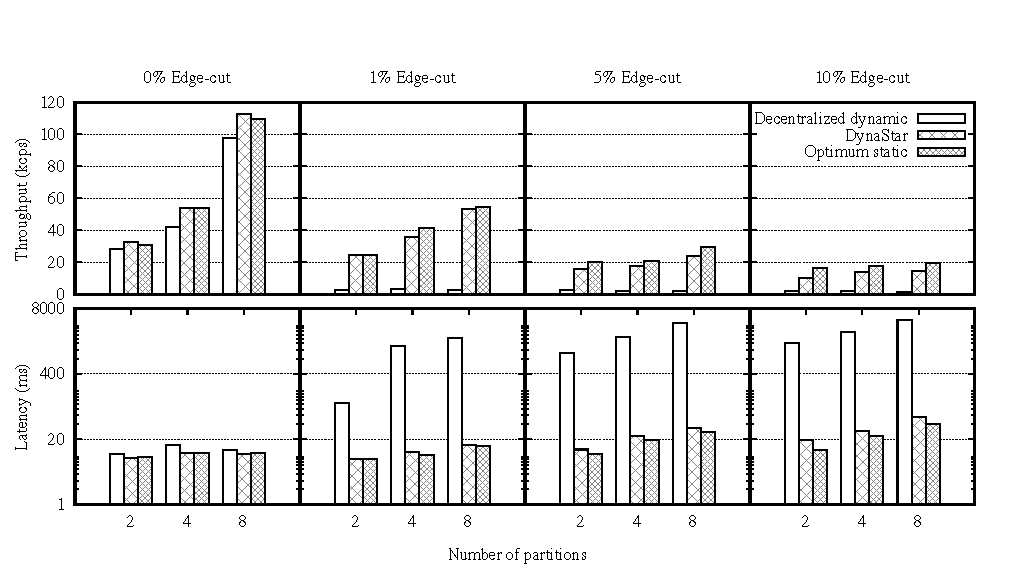
\includegraphics{figures/experiments/throughput-latency-avg-all}
	\caption{Throughput and latency, varying edge-cuts for different partitioning size.}
	\label{fig:varying_edge_cut}
\end{figure*}



\paragraph*{Performance metrics}
%
The latency was measured as the end-to-end time between issuing the
command, and receiving the response.  Throughput was measured as the
number of posts/second that the clients were able to send.

\paragraph*{Operational parameters}
%
With post commands, the frequency of single-partition
vs. multi-partition commands depends on the number of partitions, the
geometry of the social graph, and the technique used to partition the
data. We ran experiments with 2, 4, and 8 partitions.  To vary the
geometry, we generated graphs with varying percentages of edge-cuts as
computed by METIS on a static graph. Our experiments used graphs with
0\%, 1\%, 5\% and 10\% of edge cuts. We let METIS optimize the partitioning
to keep the size of the most unbalanced partition up to 30\% more than the average
partition size, that gives flexibility to decrease more the edge-cuts.
As already mentioned, we compared 
three strategies: \ssmr{}, \dssmr, and \dynastar.


\subsection{\dynastar vs. alternative systems}
\label{sec:evaluation:results}

Figure~\ref{fig:varying_edge_cut} shows the throughput and latency of the three strategies, as we vary the number of partitions for social networks with different percentages of edge cuts.

All three techniques perform similarly on experiments with
strong locality, because there are no cross-partition commands after
the graph is perfectly partitioned and no more moves occur in
\dynastar or \dssmr, and no synchronization among partitions is
necessary for \ssmr.
Consequently, all three schemes scale remarkably well.
Although \dynastar and DS-SMR have comparable performance, they differ in an important way. 
As shown in Figure~\ref{fig:motivation} (top left graph) for 4 partitions, \dynastar converges to maximum throughput after 30 seconds from the beginning of the execution, while it takes DS-SMR (decentralized dynamic scheme) about 90 seconds to converge.

With social networks that exhibit weak locality (edge cut percentage greater than zero) \dssmr\ performance decreases significantly.  
This happens because with weak locality, objects in \dssmr\ are constantly being moved back and forth between partitions without converging to a stable configuration (see also Figure~\ref{fig:motivation}, graph on the bottom right, for 4 partitions). 
In contrast, for \dynastar and \ssmr with an optimized partitioning, we see that the throughput scales with the number of partitions up to 10\% of edge cuts. 
With 10\% of edge cuts and above, the overhead from moves (in \dynastar) and cross-partition commands (in S-SMR) outweight the gains from additional partitions.

\begin{figure}[ht]
	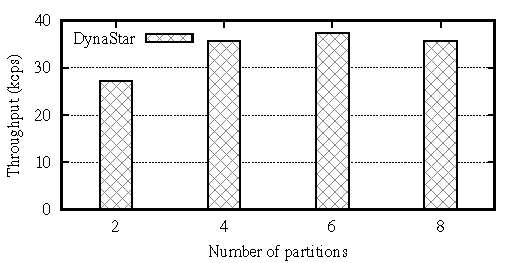
\includegraphics{figures/experiments/throughput-avg-vary-partition}
	\caption{Performance of social graph with increasing partitions.}
	\label{fig:4p1p_varying_partition_size}
\end{figure}

\begin{figure*}[h!]
  \centering
  \begin{subfigure}[b]{0.45\textwidth}
    \centering
    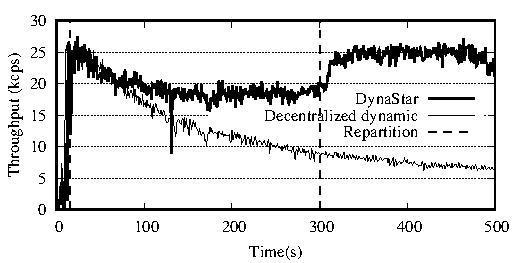
\includegraphics[width=0.95\columnwidth]{figures/experiments/dynamicload-tp-move-4p}
    \caption{\dynastar versus decentralized dynamic strategy (DS-SMR)}
  \end{subfigure}
  \begin{subfigure}[b]{0.45\textwidth}
    \centering
    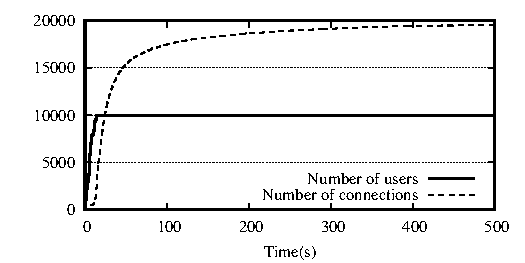
\includegraphics[width=0.95\columnwidth]{figures/experiments/dynamicload-graph-structure}
    \caption{The creation of a social network graph}
  \end{subfigure}
    \caption{Performance under dynamic workload.}
	\label{fig:dynamic_load_tput}
\end{figure*}

We can draw similar results about the latency of the three strategies (Figure~\ref{fig:varying_edge_cut}, graphs on the bottom).
The large number of move operations in DS-SMR with social graphs that cannot be perfectly partitioned result in increased latency.


\subsection{The ideal number of partitions}
\label{sec:evaluation:results}

While in the previous section we considered executions with a fixed percentage of edge cuts as we increased the number of partitions (by adjusting the social graph clustering coefficient), we now consider a fixed graph and vary the number of partitions.
Increasing the number of partitions with a fixed graph introduces a tradeoff.
On the one hand, additional partitions improve performance as there is more resources to execute posts.
On the other hand, the number of edge cuts augments with the number of partitions, which hurts performance as there are additional moves.
We evaluate the performance of \dynastar when subject to this tradeoff. 

Figure~\ref{fig:4p1p_varying_partition_size} shows that throughput scales with the number of partitions up to 6 partitions.
For each configuration, we computed the percentage of edge cuts and found that for 2, 4, 6 and 8 partitions the percentages were respectively 
0.13\%, 1.06\%, 2.28\% and 2.67\%.
Notice that only post operations are subject to this tradeoff since they may involve multiple partitions.
As discussed before, getTimeline, the most common operations in social networks, are all single-partition operations in our application and as a consequence scale linearly with the number of partitions.


\subsection{Performance under dynamic workloads}

Figure~\ref{fig:dynamic_load_tput} (left) depicts dynamically repartitioning
on-the-fly.  We started the system with an empty graph. Then clients
continuously create users and connections between them during the experiment
(running the follow command).  
The rate at which users and connections are created is shown in Figure~\ref{fig:dynamic_load_tput} (right).
The oracle monitors changes in the
graph's structure and was configured to trigger a repartitioning after all users were in the system and after 300 seconds into the execution.
%when the number of changes exceed a threshold.  
Each time the repartitioning took place, the partitioning became better and helped the throughput increase.
We also show the behavior of decentralized dynamic strategy.
When few connections are in the system, most posts are single-partition commands, but as connections are added, moves are needed to execute posts and performance decreases quickly.

%\begin{figure}[ht]
%	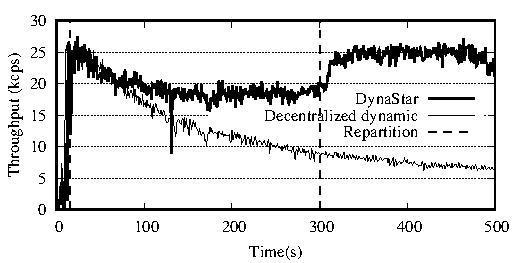
\includegraphics{figures/experiments/dynamicload-tp-move-4p}
%	\caption{Adding nodes and repartitioning dynamically}
%	\label{fig:dynamic_load_tput}
%\end{figure}
%\begin{figure}[ht]
%	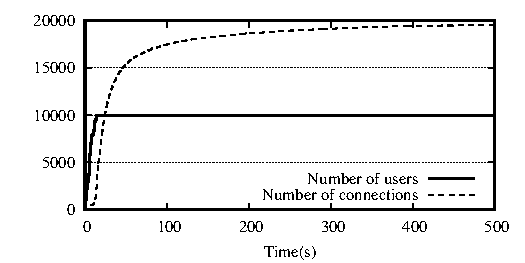
\includegraphics{figures/experiments/dynamicload-graph-structure}
%	\caption{Changes in dynamic workloads}
%	\label{fig:dynamic_load_changes}
%\end{figure}

\subsection{The performance of the oracle}

\dynastar differs from \dssmr\ in that it uses a centralized oracle
that maintains a global view of the workload graph. This oracle allows
\dynastar to make better choices about data movement, resulting in overall
better throughput and lower latency. However, introducing centralized
components in a distributed system is always a cause for some skepticism,
in case the component becomes a bottleneck. We therefore conducted two
experiments to evaluate if the \dynastar oracle is a bottleneck to
system performance. The results show that the load on the oracle is
low, suggesting that \dynastar scales well.


The first experiment assesses the scalability of the static METIS algorithm
in isolation. We measured the time to compute the partitioning solution, and
the memory usage of the algorithms for increasingly large graphs. 
The results, depicted in Figure~\ref{fig:metis_size_time}, show that METIS scales
linearly in both memory and computation time on graphs of up to 10 million vertices.

\begin{figure}[ht!]
  \centering
    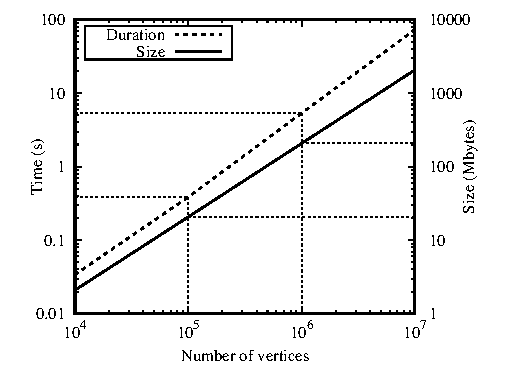
\includegraphics[width=\columnwidth]{figures/metis_size_time}
	\caption{METIS processor and memory usage.}
	\label{fig:metis_size_time}
\end{figure}

The second experiment evaluates the oracle in terms of CPU load over
time, for varying numbers of partitions. The results are shown in
Figure~\ref{fig:cpu_oracle}. The plot shows that load is higher in the
beginning of the experiment, when the clients had not yet cached the
requests and the oracle was busy moving state. However, the load diminishes rapidly, and remains relatively
low over time. This is because access to the oracle is necessary only
when clients have an invalid log or when a repartition happens. This experiments
suggest that the oracle would not become a bottleneck for reasonably large
deployments.

\begin{figure}[ht]
	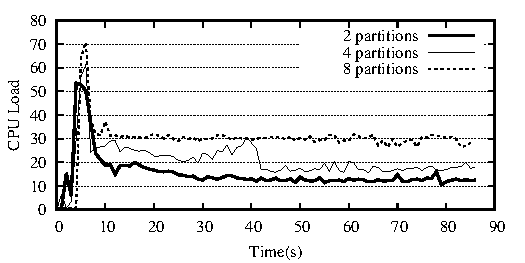
\includegraphics{figures/experiments/oracle-load}
	\caption{CPU load in the oracle.}
	\label{fig:cpu_oracle}
\end{figure}

